\chapter{Fundamentals and Related Work\label{cha:relatedwork}}

\section{Image Classification using Deep Learning}

\acrfull{dl} has a lot of advantages compared to the other \acrshort{ml} methods. First,
in many cases, it does not need a thorough and careful Feature Extraction, the techniques
such as \acrshort{cnn} help the network learn the features by itself during the training.
Second, the multiple-layer nature enable it to learn multiple levels of features from the
data. Because of that, Image Classification has been a very common domain application for
Deep Learning since the beginning, and is one of the domains where it achieved the most so
far. 

In Computer Vision, different works are usually evaluated on some standard "de facto"
labeled datasets. The accuracies on those datasets are considered as the performance
metric of a network; and those having higher scores on the datasets are considered the
better ones. ImageNet \cite{imagenet} is currently the biggest and most popular Object
Image Database available, consisting of millions of images and over 20000 object
categories. 

At the moment, there are many different approaches of Deep Learning to solve the ImageNet
Image Classification challenge. A common point of all of them is the use of the pattern
Convolutional, Max-Pooling and ReLU layers. In this section we briefly summarize the three
most popular networks which are AlexNet \cite{alexnet}, VGG \cite{vgg} and Inception
\cite{inception1, inception2, inception3}.

\begin{figure}[h]
  \centering
  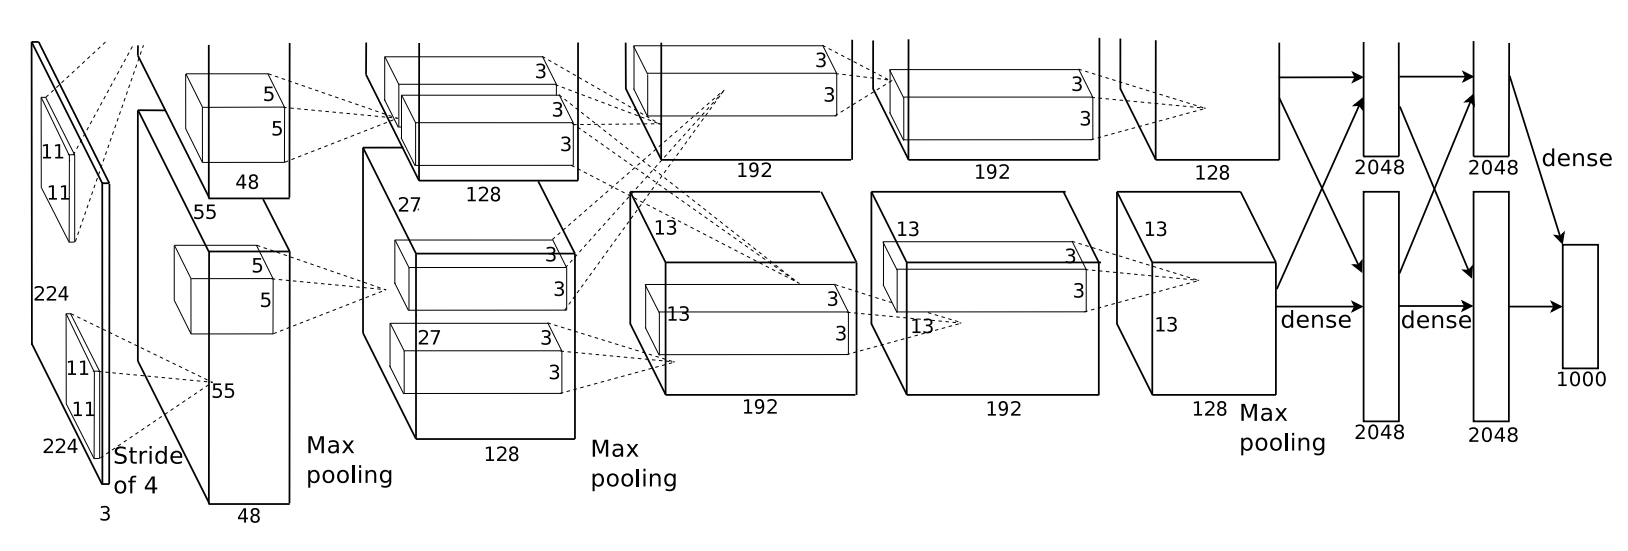
\includegraphics[width=0.9\textwidth]{alexnet_architecture}
  \caption{AlexNet Architecture \cite{alexnet}}
  \label{fig:alexnet}
\end{figure}

On ImageNet, Krizhevsky et al. \cite{alexnet} trained an 8-layer Convolutional Neural
Networks which achieved 37.5\% Top-1 error rate and 17.0\% Top-5 error rate. The network,
which is often referred as AlexNet later, was one of the first Deep Neural Networks to
improve the classification score on ImageNet significantly, and started an era that Deep
Learning leaves most of the traditional Computer Vision methods far behind. 

AlexNet consists of 8 layers as shown in Figure~\ref{fig:alexnet}. There are 5
convolutional layers and 3 fully-connected layers. The last layer is connected to a
1000-way Softmax layer because the ImageNet dataset \cite{imagenet} used to train the
network contains 1000 classes. There are different implementations on the network in
different platforms, and there are also many researches inferring the architecture, which
create small varieties of AlexNet architectures. Those differences are usually about the
size of the filters and the number of convolutional layers.

After AlexNet, there were a lot of efforts from different research groups on further
improving the classification results, resulting in many different architectures. A famous
example is VGG Net \cite{vgg}. It was introduced at the Visual Geometry Group in Oxford
and was able to achieve a Top-1 error rate of 23.7\% and Top-5 error rate of 6.8\% on
ImageNet in the best setting. The difference between VGG and AlexNet is in the filter size
and the depth of the network, which can be seen in figure \ref{fig:vgg}. Unlike AlexNet,
the authors of VGG propose a stack of three fixed filter size of $3 \times 3$ and
introduce much deeper architectures. Depending on the particular configuration, the
network can grow up to 19 layers. Despite the highly achieved ImageNet accuracies, VGG
also has big advantages which are the training time and the storage size of the network,
because of the huge depth.

\begin{figure}[h]
	\centering
	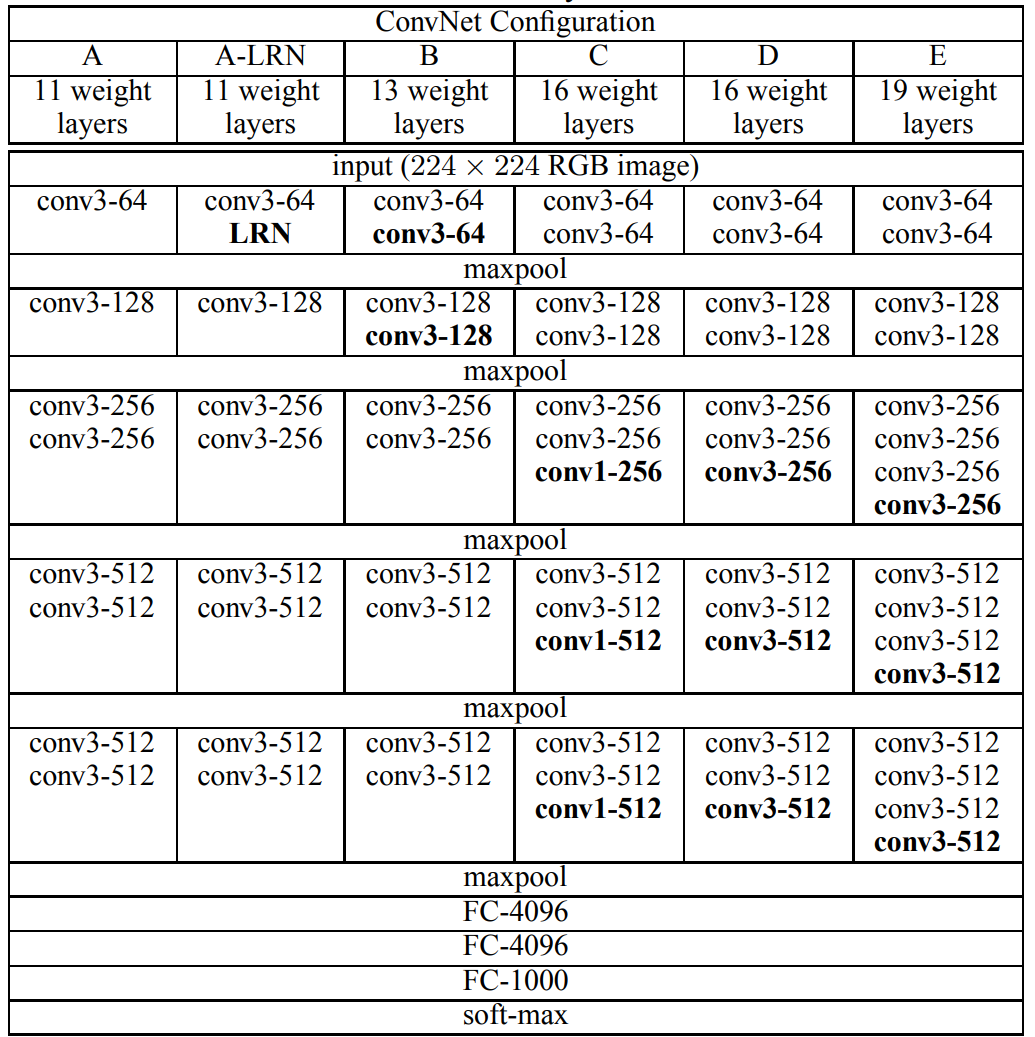
\includegraphics[width=0.8\linewidth]{vgg}
	\caption{VGG architecture and specs from the original paper \cite{vgg}}
	\label{fig:vgg}
\end{figure}

Another popular State-Of-The-Art image classification architecture is Inception
\cite{inception1}. It has quite a different design than the other two. Particularly, the
authors define a module called "Inception" and apply it multiple times in the network. As
being shown in Figure~\ref{fig:inception_module}, it uses different convolution filters at
different scales and a Pooling layer, all followed by a concatenation operation. The $1
\times 1$ convolution acts as a dimensionality reduction layer. In the overall network, a
few Inception modules are used together with other common layers such as
Convolution-MaxPool and Softmax, resulting in a network with totally 22 layers. With some
different improvements in the follow-up papers \cite{inception2, inception3}, the
Inception-v4 version could reach a Top-1 Error of 17.7\% and a Top-5 Error of 3.8\% on
ImageNet. 

\begin{figure}[h!]
	\centering
	\begin{subfigure}{0.7\textwidth}
		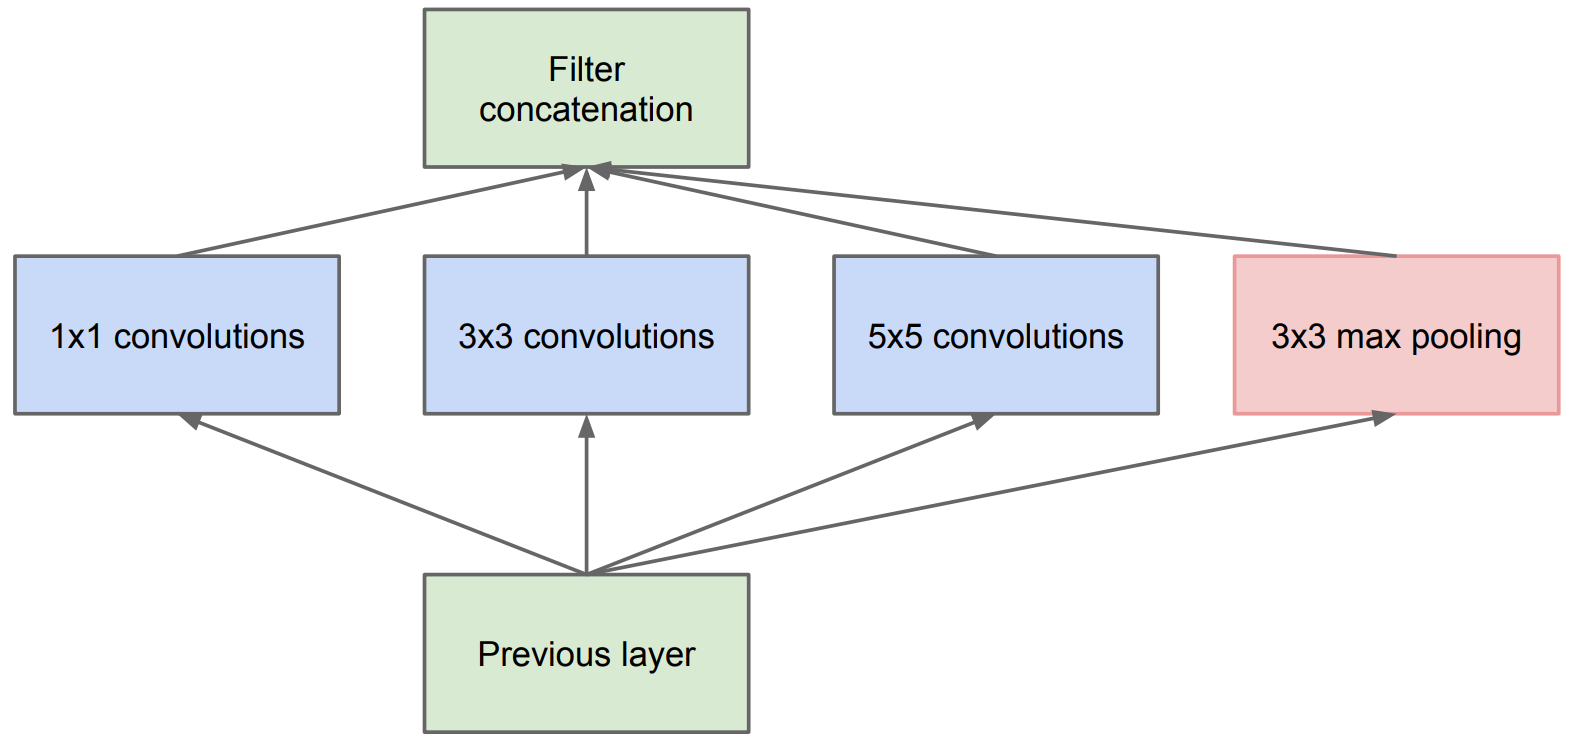
\includegraphics[width=\textwidth]{inception_module_naive}
		\caption{Inception module, naive version}
	\end{subfigure}
	\begin{subfigure}{0.7\textwidth}
		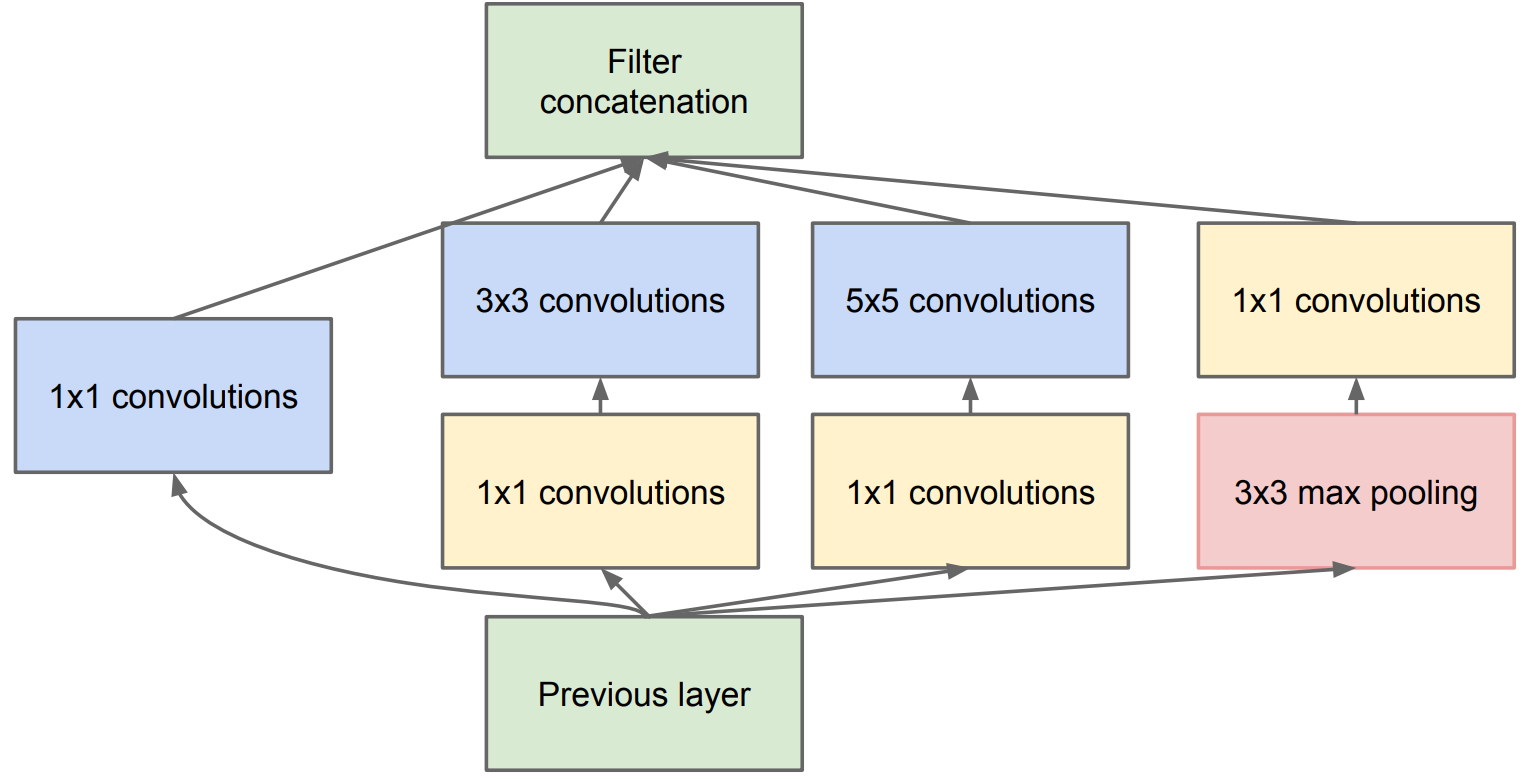
\includegraphics[width=\textwidth]{inception_module_dr}
		\caption{Inception module with dimensionality reduction}
	\end{subfigure}
	
	\caption{Inception Module from the original paper \cite{inception1}}
	\label{fig:inception_module}
\end{figure}

A common point of the three designs is that every network has a variety of different
configurations, creating different versions of the same design. People usually pick one
setting depending on the problems and the hardware power.

\subsection{Transfer Learning}

If we take a closer look at a Deep Classification Network such as AlexNet \cite{alexnet},
we can see that the last layer is often a Softmax layer, which converts the output to the
range $[0, 1]$ so that we have a prediction probability of each class. The real
classification work is done in the previous layer (fc8), where the probability that the
object image belongs to each class is calculated by a Linear Regression. In AlexNet, as we
have 1000 classes, we have 1000 neurons in fc8 corresponding to 1000 Linear Regressions.
The intuition here is that, the input of that decision layer is a good representation of
the data if the network is performing well. In principle, we can reuse the output of the
layer before fc8, which is fc7, in other \acrshort{ml} tasks.  That forms the basic idea
of Transfer Learning, which is the essential method of a number of State-Of-The-Art Object
Classifiers.

\subsection{Washington RGB-D Dataset}
\label{subsec:washington_dataset}

Beside ImageNet, the Washington RGB-D Object dataset is another one which is often used as
a "de facto" of benchmarking an Image classifier.  It is a big Image dataset introduced by
Lai ei al. \cite{washington_rgbd} at the University of Washington in Seattle. The
advantage of this dataset is that it provides depth information alongside with RGB images.
Furthermore, the RGB-D dataset is very structurally organized. Particularly:

\begin{itemize}
	\item It contains 300 common indoor objects in 51 different categories, 45 of which
		are shown in Figure~\ref{fig:washington_dataset}.
	\item Each category is then divided into different instances. For instance, in the
		"Apple" category there are 5 different apples shown in
		Figure~\ref{fig:apple_washington}.
	\item Each instance is recorded in 3 360\degree sequences by 3 different camera
		angles: 30\degree, 45\degree, and 60\degree.
	\item Each frame has:
		\begin{itemize}
			\item an RGB image of the object
			\item a Depth map
			\item a Mask indicating the	object position for extracting the object without
				background (which we do not use in this project)
			\item For every 5th frame, there is an estimated pose.
		\end{itemize}
\end{itemize}

\begin{figure}[h]
	\centering
	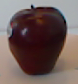
\includegraphics[height=0.10\textheight]{apple_1_1_1_crop}
	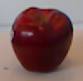
\includegraphics[height=0.10\textheight]{apple_2_1_1_crop}
	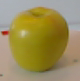
\includegraphics[height=0.10\textheight]{apple_3_1_1_crop}
	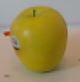
\includegraphics[height=0.10\textheight]{apple_4_1_1_crop}
	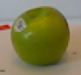
\includegraphics[height=0.10\textheight]{apple_5_1_1_crop}
	\caption{5 different instances of the "Apple" category in the Washington RGB-D object dataset}
	\label{fig:apple_washington}
\end{figure}

\begin{figure}[h]
	\centering
	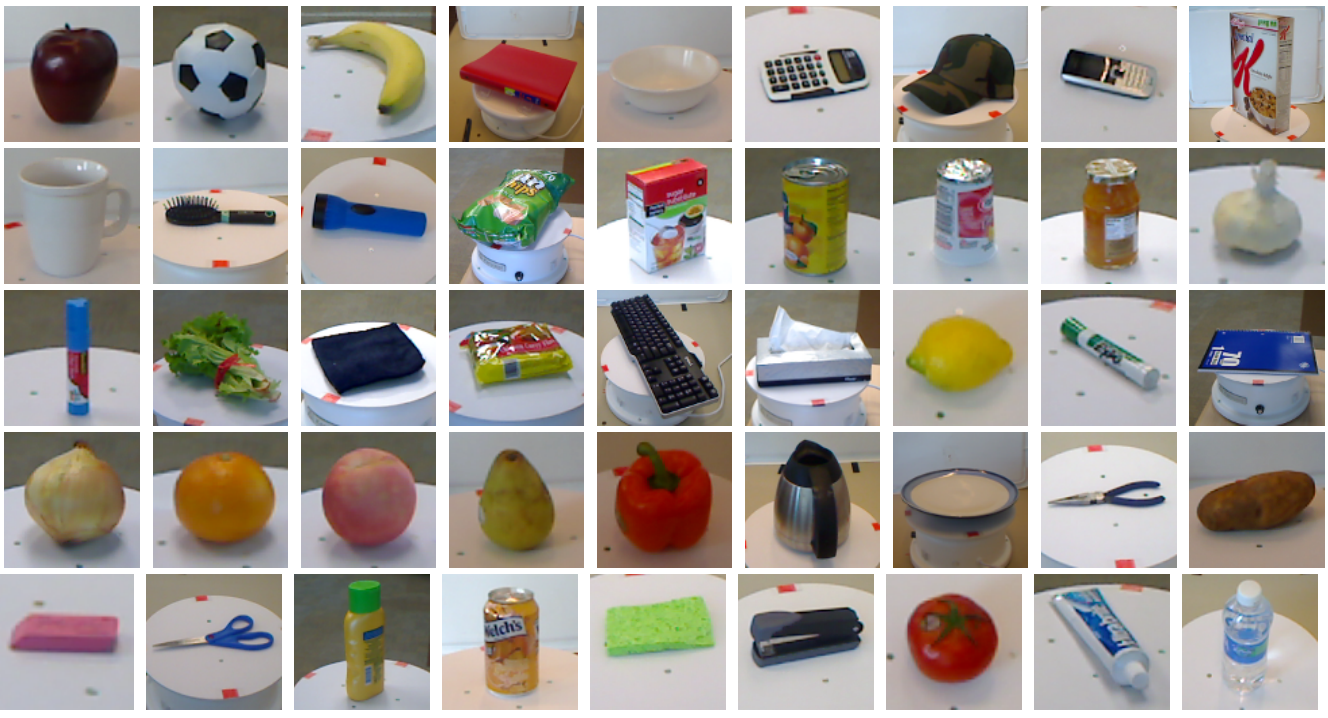
\includegraphics[width=0.8\linewidth]{washington_dataset}
	\caption{Sample RGB Images from the dataset \cite{washington_rgbd}. Each object belongs to a different
		category. Figure from the original paper. }
	\label{fig:washington_dataset}
\end{figure}

\subsection{Object Recognition on Washington RGB-D dataset}

As we have discussed in section \ref{subsec:washington_dataset}, the Washington RGB-D
Dataset has some advantages over the other ones as a "de facto" benchmarking dataset. The
biggest one is the depth maps provided alongside with the RGB frame of each item which
enables researchers to explore the potential of depth information in different
\acrshort{ml} tasks. 

The earliest work on the RGB-D Object Dataset came from the authors of the dataset
themselves \cite{lai_recognition}. They apply \acrfull{hog} to both the RGB frame and the
Depth map and propose a distance metric among different instances to do some
classifications. They achieved an accuracy of 85.4\% on the category classification task,
which was the State-Of-The-Art before the \acrshort{cnn} era.

Soon after \acrshort{cnn} was introduced, it surpassed all other traditional Computer
Vision methods. Together with the Transfer Learning techniques, the researchers quickly
got very high results on the RGB-D Object Dataset and demonstrate that depth data does
indeed reduce the classification errors \cite{eitel, alexandre}. The differences between
different approaches are usually about which pre-trained networks the authors use and how
they pre-process the image channels, especially the depth channel. In this thesis, we
build our baseline classifier based on the main components from Eitel et al.  \cite{eitel}
as it achieved high accuracies on the same dataset and the architecture is simple enough
to not take too much time to train, which is very important because we also have to train
other bigger networks (\acrshort{gan}s).

Transfer Learning is the main component of Eitel et al. \cite{eitel}. In the paper, the
authors use an implementation of AlexNet in Caffe (CaffeNet) to get the representations of
the objects in the Washington RGB-D dataset \cite{washington_rgbd}. Particularly, there
are two channels of AlexNet, one is for the RGB and the other one is for the depth-map.
The Depth-map is colorized using the jet color-map before feeding into AlexNet. The
outcome representations of both channels are then fed into a fully-connected layers, where
the final results are connected to a 51-way Softmax layer, to classify 51 different
classes in the Washington Object Dataset \cite{washington_rgbd}. Figure
\ref{fig:eitel_net} describes the network.

\begin{figure}[h]
  \centering
  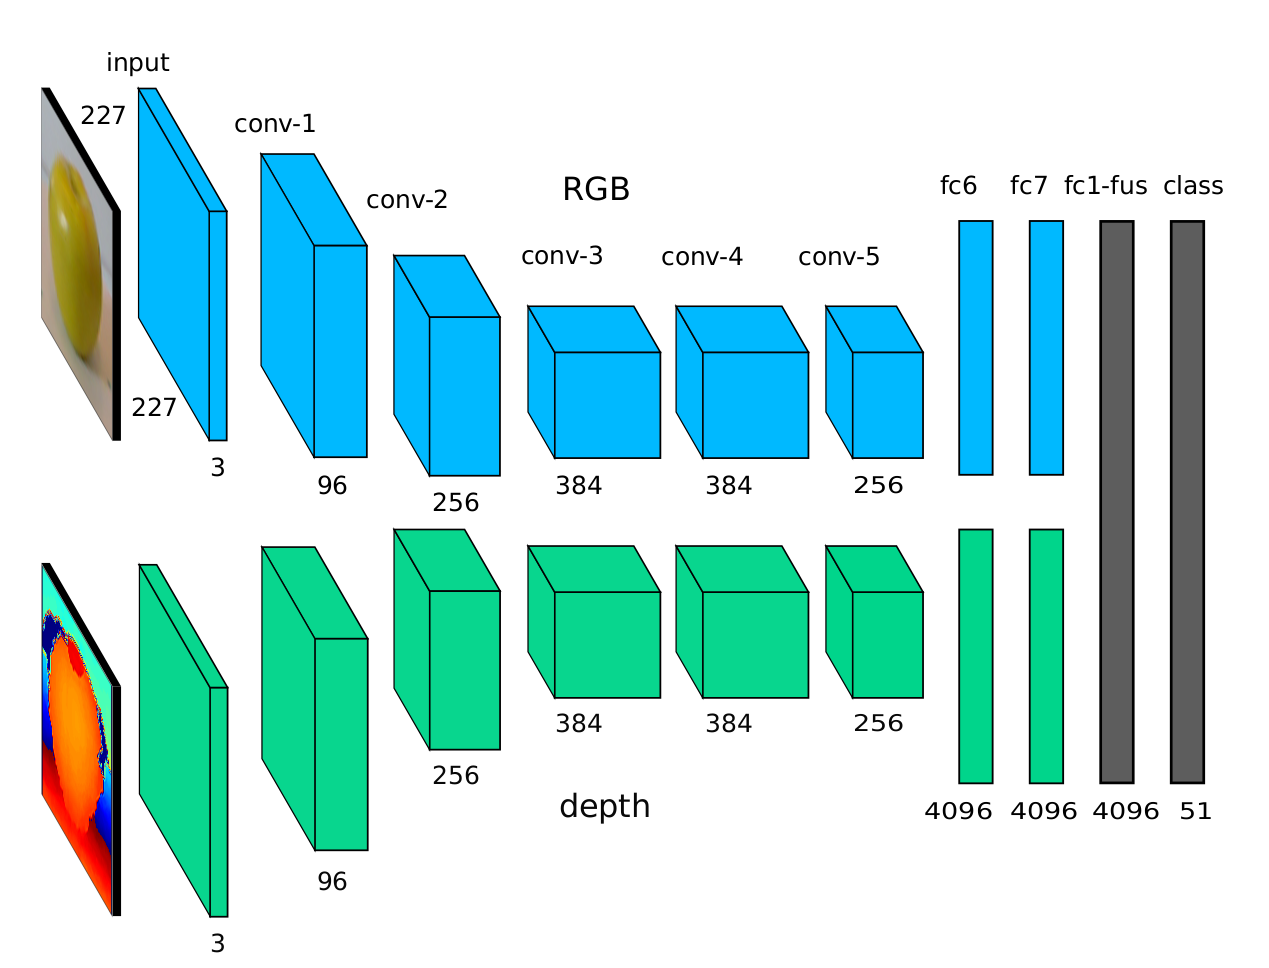
\includegraphics[width=0.8\textwidth]{eitel_net}
  \caption{Eitel et al. architecture for Object Classification. Figure from the original
	  paper \cite{eitel}}\label{fig:eitel_net}
\end{figure}

\section{\acrfull{gan}}

As being already mentioned in section \ref{subsec:intro_gan}, \acrshort{gan} consists of
two differentiable and adversarial functions: the Generator and the Discriminator, usually
in different forms of Deep Neural Networks.  

There can be different designs for the two networks depending on the domains that
\acrshort{gan}s are applied. In Computer Vision applications, it is common that the
Generator is a \acrfull{cnn} which behaves in a similar way as how an Auto Encoder
\cite{auto_encoder} works. The first half is an Encoder where an image is reduced to a
representation of 1D array, then the second half tries to decode that representation to
the original image. The difference here is that this Generator does not minimize the
direct loss between the output and the input. Instead, it tries to maximize the loss of
the Discriminator. The Discriminator, as already been explained in section
\ref{subsec:intro_gan}, is a binary classifier who tries to distinguish the original image
and the output image from the Generator. 

In the most basic setting, the Discriminator always receives a pair of inputs:

\begin{itemize}
	\item Target: The ground-truth from the dataset, also called "Real Item", label 1
	\item Output: The product of the Generator, also called "Fake Item", label 0
\end{itemize}

Let $G$ denote the generating function and $D$ denote the classification function, and
given an arbitrary image $x$, then $G(x)$ is also an image and $D(x)$ is a scalar label
where $D(x) \in {0, 1}$.

Obviously, the goal of the Discriminator is to assign label 1 for all the real images and
label 0 for all the fake images. Thus the Discriminator Loss is a Cross-Entropy between
the output of the Discriminator and the set of labels ${0, 1}$. In other words, the
Discriminator maximizes the probability of assigning the correct labels to its inputs by
maximizing the Value Function $V(D) = \log(D(x)) + \log(1 - D(G(z)))$.

At the same time, the goal of the Generator is to "create troubles" for the Discriminator.
Particularly, it tries to make the Discriminator think that its output is "real" (label
1), meaning it minimizes the second component of the Discriminator Value Function $\log(1
- D(G(z)))$.

Based on the setting above, we end up in a two-player minimax game with the 
following value function:

\begin{align*}
	\min_{G} \max_{D} V(D, G) = \mathbb{E}_{x \sim p_{data}(x)} [\log D(x)] +
	\mathbb{E}_{z \sim p_z(z)}[\log(1 - D(G(z)))]
\end{align*}

In practice, for implementation purpose, people usually set the Discriminator Loss to be
$L(D) = -V(D, G)$ so that we can use Gradient Descent to minimize it and utilize the
existing Deep Learning frameworks. The Generator is also set to maximize $\log(D(G(z)))$,
equivalent to minimizing $-\log(D(G(z)))$, instead of minimizing $\log(1 - D(G(z)))$
because the latter has problems of vanishing gradients, shown in \cite{gan}.

We can see that the Discriminator job is as simple as any other binary classifier, it
distinguishes the real data distribution $p_{data}$ from the Generator outcome
distribution $p_{g}$. In order to "fool" it, the Generator has to learn the data
distribution $p_{data}$. In every step, the optimal Discriminator is $D^{*}(x) =
\frac{p_{data}(x)}{p_{data}(x) + p_{g}(x)}$, proved in \cite{gan}. When the system reaches
an equilibrium, $p_{g}$ should converge to $p_{data}$, thus the optimal Discriminator
Outcome should be $D^*(x) = 0.5$, equivalent to a Value Function with absolute value
$|\log(0.5)+ \log(0.5)| = 1.38629436112$. This is an important property that we can use to
determine if the \acrshort{gan} training has converged or not.

As an example, if we want to learn an apple image distribution, the Generator will draw
synthesized apple images from an arbitrary input $z$, and the Discriminator will try to tell
that the output apple image is a "fake" one and an arbitrary image from the data is a "real"
one. When the two networks converge, we should have an implicit model representing an apple
image distribution.

\section{Conditional \acrshort{gan} and Pix2pix}

The original non-conditional \acrshort{gan} is sometimes referred as the "Vanilla
\acrshort{gan}". It sets up a good foundation for the field, but is sometimes unstable and
hard to train. In some applications, people are not interested in the general distribution
but rather pay attention to a directed data generation, that is, a conditional
distribution. For instance, generating a random apple may not be as interesting to somebody
as creating an image of "Pink Lady" apple. Just shortly after the introduction of
\acrshort{gan}, Mirza and Osindero \cite{cogan} proposed Conditional GANs, an improved
version of \acrshort{gan}. The idea is simple, instead of generate from an arbitrary noise
input $z$, the Generator also takes another vector $y$ as the condition. In the example of
apple image generation, we can provide a green apple image, a string "Green Apple", or a binary
label vector as $y$. The Discriminator also takes $y$ as its condition. By being trained
in that way, \acrshort{gan} now learns a conditional model $p_{g}(x|y)$ and tries to make
it as close to the conditional distribution of the data $p_{data}(x|y)$ as much as
possible. Figure \ref{fig:co_gan_model} demonstrates how conditional \acrshort{gan} works.

\begin{figure}[h]
	\centering
	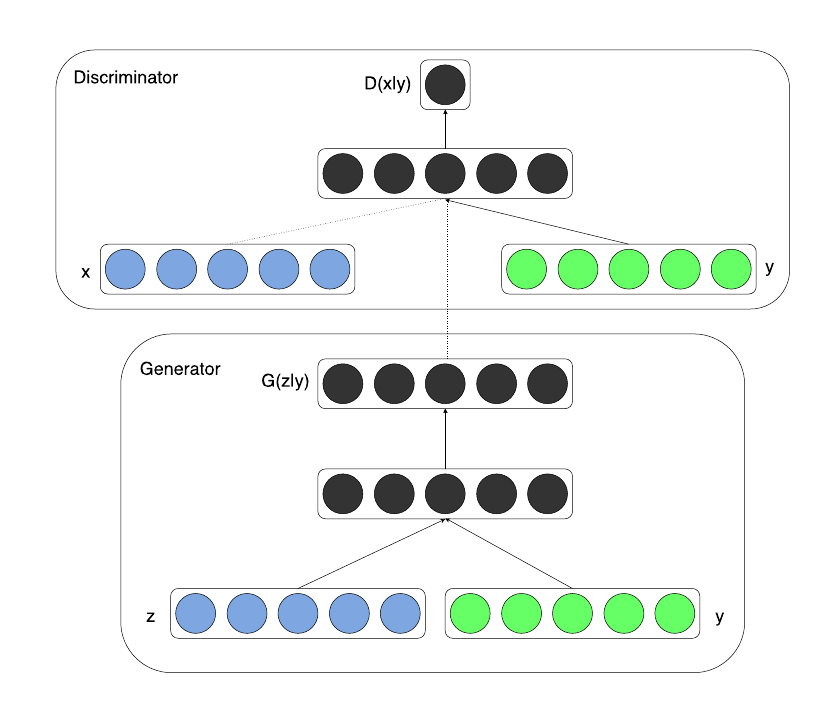
\includegraphics[width=0.5\linewidth]{img/co_gan_model}
	\caption{Conditional \acrshort{gan}s. Figure from original paper \cite{cogan}}
	\label{fig:co_gan_model}
\end{figure}

Conditional \acrshort{gan}s have many applications, one of them is image super-resolution.
The idea is to sharpen low-resolution image by converting it to a higher-resolution one.
In SRGAN \cite{sr_gan}, shown in Figure~\ref{fig:sr_gan_example}, the Generator takes a
downsampled image as the input condition and produces a higher-resolution image through a
convolutional network with some skip connections and upscaling layers; and the
Discriminator distinguishes the original input image from the output of the Generator
while being conditioned on the same downsampled image. The results were more realistic
than the other State-Of-The-Art methods, as being shown in
Figure~\ref{fig:sr_gan_example}.

\begin{figure}[h!]
	\centering
	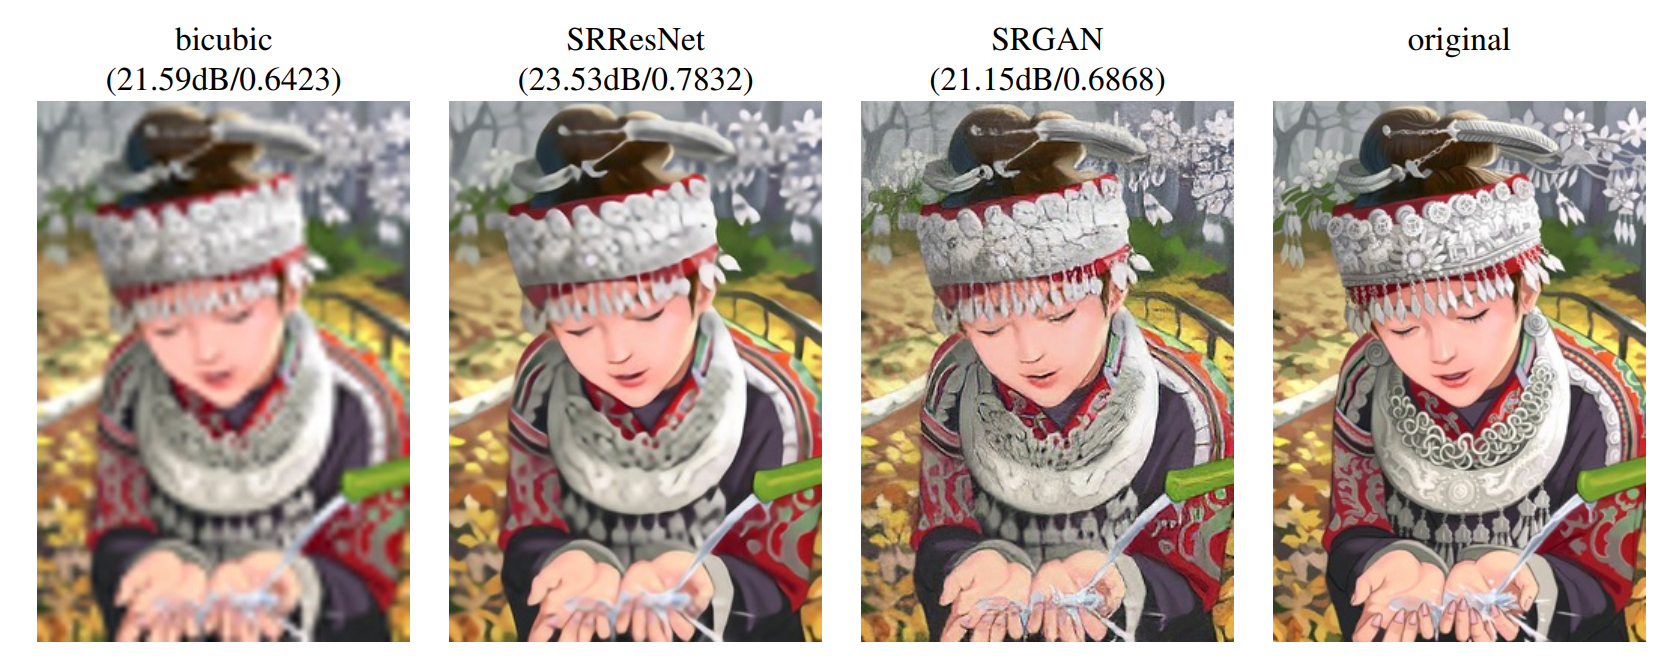
\includegraphics[width=0.8\linewidth]{sr_gan_example}
	\caption{Examples from SRGAN \cite{sr_gan}}
	\label{fig:sr_gan_example}
\end{figure}

\acrfull{pix} \cite{pix2pix} is another conditional \acrshort{gan}. It maps an image to
another image. The authors demonstrate that \acrshort{pix} is able to generate satellite
images from map views and vice versa, detailed buildings with texture from skeleton
sketches, or day to night transformation. Those impressive results come from the idea of
conditioning a \acrshort{gan} on an input image. In figure \ref{fig:pix2pix_examples}, we
can see some outputs of \acrshort{pix} from the authors.  The general workflow is
demonstrated in Figure~\ref{fig:pix2pix_workflow}.

\begin{figure}[h!]
	\centering
	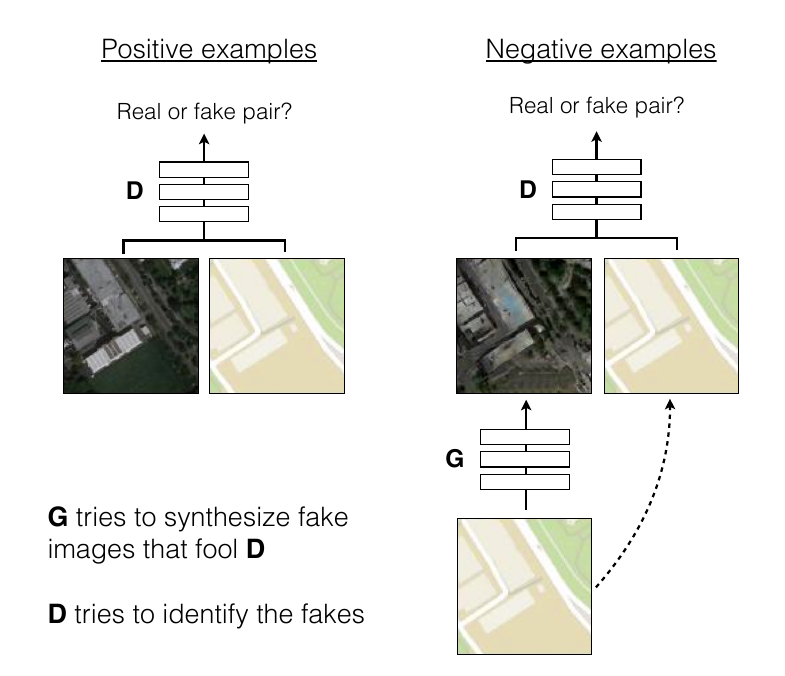
\includegraphics[width=0.5\linewidth]{img/pix2pix_workflow}
	\caption{How \acrshort{pix} works \cite{pix2pix}.}
	\label{fig:pix2pix_workflow}
\end{figure}

\begin{figure}[h!]
	\centering
	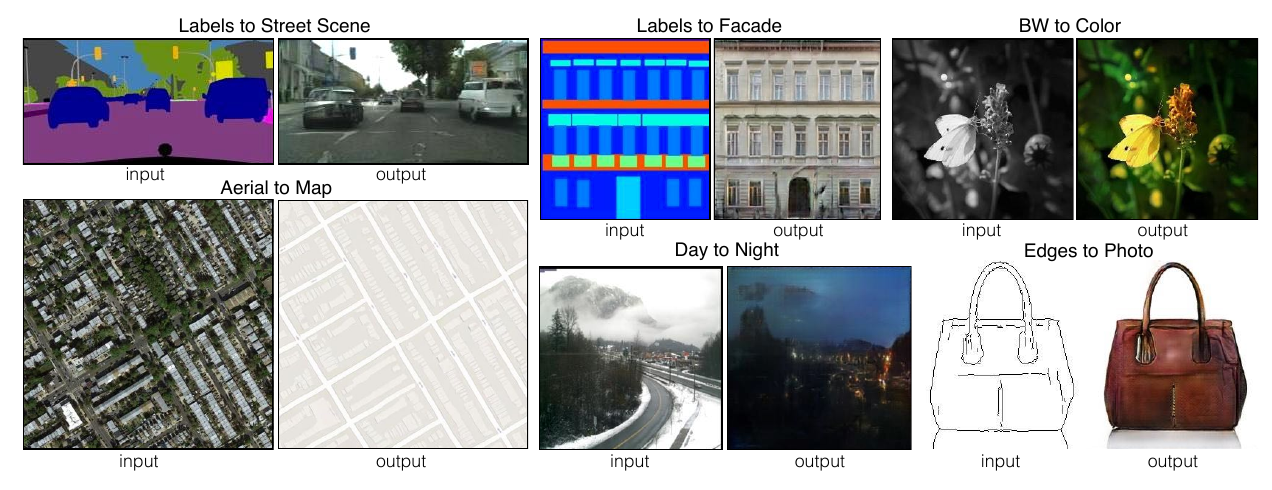
\includegraphics[width=0.8\linewidth]{img/pix2pix_examples}
	\caption{Examples of generated images from \acrshort{pix} \cite{pix2pix} }
	\label{fig:pix2pix_examples}
\end{figure}

As this is a conditional \acrshort{gan}, the loss function is also a little bit different
from the Vanilla \acrshort{gan} in the sense that all the components now are conditional
on an image $y$.  Besides, the authors also suggest using an L1 loss to boost up the
Generator training as it helps the Generator learn faster and L1 enforces less blurry
images than L2.

\begin{align*}
	\min_{G} \max_{D} V(D, G) = \mathbb{E}_{x \sim p_{data}(x)} [\log D(x, y)] +
	\mathbb{E}_{z \sim p_z(z)}[\log(1 - D(G(y, z), y))] \\ 
	+ \lambda L1(G)
\end{align*}

